\chapter{بررسی نهایی}
نتیجه‌های بدست آمده در دو بخش قبلی، کارایی تی‌اس‌ان‌ای را بر روی چندین مجموعه مختلف از دیتاست‌ها به خوبی نشان داد. در این بخش قصد داریم تا تی‌اس‌ان‌ای را با چندین تکنیک مطرح دیگر مقایسه کنیم و تفاوت‌های آن را بیان نماییم. همچنین به برخی از نقاط ضعف تی‌اس‌ان‌ای اشاره کرده و مواردی را برای ارتقای این روش ارائه می-کنیم.

\section{مقایسه با دیگر تکنینک‌ها}

امروزه پیروش
مقیاس بندی کلاسیک\LTRfootnote{ classical scaling }
که بسیار نزدیک به ‌$pca$ است، به دنبال یک انتقال خطی می‌گردد که مجموع مربعات خطاها\LTRfootnote{SSE} را مینیمم کند. خطاها به صورت فاصله‌ی دو به دوی داده‌ها در فضای بالاتر و تبدیلشان در فضای پایین تر تعریف می‌شوند. یک مدل خطی مانند مقیاس بندی کلاسیک، نمی‌تواند خوشه‌های منحنی مانند را به خوبی مدل کند، چراکه تمرکز آن بیش‌تر بر روی حفظ فاصله‌ی داده‌های جدا از هم است و توجهی به حفظ فاصله‌ی داده‌ی نزدیک به هم ندارد. یک روش مهم که سعی در بر طرف کردن مشکلات مقیاس بندی کلاسیک دارد، روش نقشه برداری 
سامون\LTRfootnote{sammon} 
می‌باشد که تابع هزینه را به صورت تقسیم فاصله‌ی اقلیدسی دو به دوی داده‌های انتقال داده شده به فاصله‌ی اقلیدسی آن‌ها در فضای اصلی تعریف می‌کند. بنابراین تابع هزینه برابر خواهد بود با فرمول \cref{chapfig4}
\begin{figure}
	\centering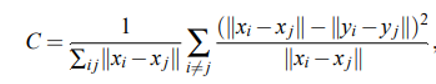
\includegraphics[scale=.6]{chapfig4.PNG}
	\caption{ }\label{chapfig4}
\end{figure}

که کسر بیرون از علامت سیگما برای ساده سازی گرادیان تابع نوشته شده است. نقطه ضعف اصلی این تابع هزینه این است که حفظ داده‌های با فاصله نزدیک تا حد زیادی به اندازه فاصله دو به دوی آن‌ها وابسته است. به نحوی که اگر یک خطای کوچک در مدل سازی دو داده‌ای که بسیار به یکدیگر نزدیک هستند رخ دهد، منجر به افزایش تابع هزینه به مقدار زیادی خواهد شد. از آنجایی که تمام فواصل دو به دو در شکل دهی فرم‌های محلی نقش دارند، بهتر است تا اهمیتی تقریبا برابر به فواصل به اندازه کافی کوچک داده شود. 
\\
در مقابل روش $Sammon$، روش کرنل گوسی  \LTRfootnote{ Gaussian kernel } وجود دارد که توسط تی‌اس‌ان‌ای در ابعاد بالا به کار گرفته می‌شود. این روش یک حاشیه نرم بین فرم‌های محلی ایجاد می‌کند و برای جفت‌هایی که بر مبنای انحراف معیار مدل گوسی به یکدیگر نزدیک می‌باشند، اهمیت بیش‌تری در نظر گرفته می‌‌شود. بنابراین اهمیت حفظ هر فاصله، مستقل از بزرگی آن است. علاوه بر آن، تی‌اس‌ان‌ای تعداد همسایگان محلی را برای هر داده به طور جداگانه و بر مبنای چگالی محلی مشخص می-کند.
برتری کارایی تی‌اس‌ان‌ای در مقایسه با $Isomap$ در بحث مقاوم بودن در برابر             $"short circuiting"$ به خوبی نشان داده شد. علاوه بر آن، $Isomap$ بر روی حفظ ساختارهای بزرگ داده تمرکز دارد در حالی که تی‌اس‌ان‌ای به حفظ فرم‌های محلی بیش‌تر اهمیت می‌دهد.
عملکر قوی تی‌اس‌ان‌ای در مقایسه با $LLE$، به یک نقطه ضعف بزرگ در $LLE$ باز می‌گردد: تنها عاملی که باعث می‌شود تا تمام داده‌ها در یک خوشه قرار نگیرند محدودیتی است که بر روی کوواریانس داده‌ها انتقال داده شده اعمال می‌شود. در عمل این محدودیت می‌تواند با قرار دادن تمام داده‌ها حول یک مرکز و چندین داده‌ی متراکم که فاصله‌ی آن‌ها از مرکز به نسبت بقیه داده‌ها بسیار زیاد است به سادگی ارضا شود. محدودیت کوواریانس در گراف همسایگی نیز می‌تواند با وجود چند ناحیه متراکم و جدا از هم ارضا شود. بنابراین روش $LLE$ نمی‌تواند ناحیه‌های متراکم که شامل چند خوشه هستند ولی از یکدیگر دور اند را به خوبی مدل کند. به عنوان مثال  \cref{chapfig1} را در نظر بگیرید، $LLE$ قادر به تفکیک خوشه‌های قرمز و آبی و همچنین خوشه‌های زرد و سبز نخواهد بود و کل دیتاست را به دو خوشه دسته بندی می‌کند. 
همانند $LLE$ ، قدم زدن تصادفی در تی‌اس‌ان‌ای از گراف همسایگی استفاده می‌کند اما مشکلات $LLE$ را نخواهد داشت چراکه شباهت دو به دوی داده‌ها در فضای اصلی، با در نظر گرفتن ترکیبی از تمام مسیرهای بین دو داده در گراف همسایگی مشخص می-شود.


\begin{figure}
	\centering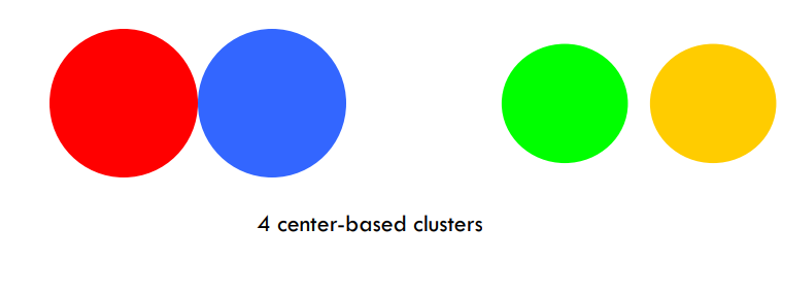
\includegraphics[scale=.6]{chapfig1.PNG}
	\caption{ }\label{chapfig1}
\end{figure}

\section{نقاط ضعف}
اگرچه در قسمت قبل مشاهده کردیم که تی‌اس‌ان‌ای نسبت به برخی روش‌های دیگر برتری هایی دارد اما این روش دارای نقطه ضعف‌هایی نیز می‌باشد که اصلی ترین آن‌ها عبارت‌اند از: (‌۱) مشخص نیست که تی‌اس‌ان‌ای در کاهش ابعاد دقیقا چگونه عمل می-کند. (۲) کاهش ابعاد بر مبنای ویژگی‌های محلی داده‌ها، باعث می‌شود تا تی‌اس‌ان‌ای نبت به ابعاد ذاتی داده‌ها حساس باشد. (۳) تابع هزینه تی‌اس‌ان‌ای محدب نیست و بنابراین تضمینی وجود ندارد که به بهینه ترین حالت برسیم. در ادامه به طور خلاصه به شرح این نقاط ضعف می‌پردازیم.
\begin{itemize}
\item 	کاهش ابعاد برای اهداف دیگر: مشخص نیست که روش تی‌اس‌ان‌ای  در حالت کلی دقیقا چگونه ابعاد را کاهش می‌دهد. این روش برای کاهش ابعاد داده‌ها به دو یا سه بعد مناسب است اما در حالتی که نیاز داشته باشیم ابعاد داده‌ها بیش‌تر از سه بعد باشد، بهتر است از آن استفاده نکنیم چراکه نمی‌تواند به خوبی داده‌‌ها را مدل کند. بنابراین اگر شرایط به گونه ای باشد که برای حفظ فرم و اطلاعات کلی داده‌ها به بیش‌تر از سه بعد نیاز باشد، تی‌اس‌ان‌ای کارایی لازم را نخواهد داشت.
\item 	نفرین ابعاد ذاتی: تی‌اس‌ان‌ای ابعاد داده‌ها بر مبنای ویژگی‌های محلی دیتاست کاهش می‌دهد که این امر می‌تواند آن را در مقابل دیتاست‌هایی که ابعاد ذاتیشان بالا است و تنوع نواحی مختلف آن‌ها زیاد است، آسیب پذیر کند. روش‌های $LLE$ و $Isomap$ هم دارای همین مشکل هستند.
\item	غیر محدب بودن تابع هزینه تی‌اس‌ان‌ای: تابع هزینه در تی‌اس‌ان‌ای محدب نمی‌باشد بنابراین تضمینی وجود ندارد که به بهینه ترین حالت ممکن برسیم چراکه باید پارامترهای بهینه سازی زیادی را بیابیم که در هر اجرا و آزمایش متفاوت خواهند بود. اما این نقطه ضعف نمی‌تواند دلیلی برای کنار گذاشتن تی‌اس‌ان‌ای و استفاده از روش‌های $LLE$ و $Isomap$ که تابع هزینه آن‌ها محدب است باشد. چراکه رسیدن به مینیمم نسبی یک تابع هزینه که ویژگی‌های داده‌ها را به وطور قابل قبولی منعکس می‌کند، بهتر از رسیدن به مینیمم مطلق تابعی است که نمی‌تواند اطلاعات مد نظر دیتاست را مدل کند. به علاوه، محدب بودن تابع هزینه به این معنا نیست که حتما می‌توان به بهینه ترین حالت ممکن رسید. چراکه محاسبه مینیمم مطلق توابع هزینه در بسیاری از تجربه‌های واقعی از نظر بار محاسباتی غیر ممکن است.
\end{itemize}

\section{نتیجه گیری}
در این مقاله، یک تکنیک جدید برای مصور سازی داده‌ها معرفی شد که می‌تواند ویژگی-های محلی داده‌های نزدیک به هم را به خوبی منعکس کند و علاوه بر آن بخشی از اصلی ترین ویژگی‌های سراسری دیتاست را نیز حفظ نماید. پیچیدگی حافظه و زمان روش تی‌اس‌ان‌ای برابر $O(n^2)$ است. اما رویکرد شاخصی در این مقاله مطرح شد که اجرای تی‌اس‌ان‌ای را بر روی دیتاست‌های بزرگ ممکن می‌کند. تجربه‌های بدست آمده از اجرای تی‌اس‌ان‌ای بر روی چندین دیتاست مختلف نشان داد که این روش به نسبت برخی روش‌های مطرح دیگر در زمینه مصور سازی داده بهتر عمل می‌کند.
برای ارتقای این روش در آینده قصد داریم تا بهینه سازی را بر روی تعداد درجات آزادی توزیع $t\-Student$ (که در تی‌اس‌ان‌ای استفاده می‌شود) پیاده سازی کنیم. این کار به برطرف کردن اولین نقطه ضعف مطرح شده در قسمت قبل کمک می‌کند. همچنین گسترش تی‌اس‌ان‌ای را به گونه‌ای که هر داده در فضای بالاتر بتواند به چندین داده در فضا پایین‌تر مدل شود، بررسی خواهیم کرد.  به علاوه، هدف ما توسعه‌ی یک نسخه پرامتری از تی‌اس‌ان‌ای است که در آن با استفاده از تابع هدف تی‌اس‌ان‌ای ، به آموزش یک شبکه عصبی چند لایه‌ای که یک نگاشت مستقیم از فضای اصلی به یک فضای با ابعاد کمتر را فراهم می‌کند، می‌پردازیم. 

